\documentclass[a4paper,10pt,twocolumn]{article}
\usepackage[utf8]{inputenc}
\usepackage[ngerman]{babel}
\usepackage{hhline}

\usepackage{acronym}
\usepackage[hidelinks]{hyperref}
\usepackage{todonotes}
\usepackage{graphicx}
\usepackage{url}
\usepackage{listings} %Quellcode einbinden
\usepackage{tabularx} %Tabellen erstellen
\usepackage{multicol} %Format text in multiple columns
\usepackage{enumitem}
\usepackage[gen]{eurosym} % Euro-Zeichen

\RequirePackage[numbers,sort&compress]{natbib}
\RequirePackage[nottoc]{tocbibind}

%macros and constants
\newcommand{\editors}{Hendrik van Essen, Arndt Tigges, Robert Munteanu}

\newcommand{\hmargin}[1]{\addtolength{\oddsidemargin}{#1}\addtolength{\evensidemargin}{#1}\addtolength{\textwidth}{-#1}\addtolength{\textwidth}{-#1}}
\newcommand{\vmargin}[1]{\addtolength{\topmargin}{#1}\addtolength{\textheight}{-#1}}

\setlength{\marginparwidth}{2cm}

%opening
\hmargin{-15mm}\vmargin{-30mm}
\addtolength{\textheight}{15mm}

\title{Smarthome 2 - Ein lokal betriebenes Sicherheitssystem für das Smart Home}
\author{\editors}
\date{}

\begin{document}

\maketitle

\section*{Abstract}
Dieses Projekt beschäftigt sich mit dem immer aktueller werdenden Thema des \textit{Smart Homes}. Die großen Anbieter dieser Systeme bieten jedoch häufig Lösungen an, die den Nutzer an bestimmte Vorgaben binden, sei es die ausschließliche Unterstützung von Geräten bestimmter Hersteller oder der Zwang zur Datenverarbeitung über die Cloud.\\
Ein System zu entwickeln, welches diese Beschränkungen nicht aufweist war Ziel dieses Projektes.\\
Um die Sicherheit des Systems und der zwischen den Systemkomponenten übertragenen Informationen zu gewährleisten, verläuft die Kommunikation und Datenverarbeitung nicht über einen nicht identifizierbaren Server, sondern findet stattdessen verschlüsselt im lokalen Netz statt.\\
Mit dem Ziel, ein offenes, erweiterbares, kostengünstiges, benutzerfreundliches und sicheres System zu entwickeln, lag das Hauptaugenmerk darauf, möglichst bereits existierende Lösungen, von Kommunikationsprotokollen, über Hardwarekomponenten bis hin zu Softwarelösungen, mit einer großen User-Community in dem Gesamtsystem zum Einsatz zu bringen, um ein zukunftsorientiertes System zusammenzustellen, das die Philosophie des Open Source Entwicklungskonzepts symbolisiert. 


\section*{Abkürzungsverzeichnis}
\begin{acronym}[LONGEST]
	%\singlespace
	\acro{CA}{Certificate Authorithy}
	\acro{ESP-IDF}{Espressif IoT Development Framework}
	\acro{openHAB}{Open Home Automation Bus}
	\acro{OTA}{Over-the-Air}
	\acro{MQTT}{Message Queue Telemetry Transport}
	\acro{TLS}{Transport Layer Security}
	\acro{HTTP}{Hypertext Transfer Protocol}
	\acro{HTTPS}{Hypertext Transfer Protocol Secure}
	\acro{RAM}{Random Access Memory}
\end{acronym}


\section{Motivation}
Derzeit gibt es auf dem Markt eine Vielzahl an Lösungen für Home Automation. In den meisten Fällen handelt es sich jedoch um Systeme, welche zwar innerhalb ihres Ökosystems gut funktionieren, aber Probleme erzeugen, sobald unterschiedliche Geräte mehrerer Hersteller genutzt werden sollen. Weiterer Nachteil der Verwendung eines geschlossenen Systems ist die Abhängigkeit vom Hersteller. Sowohl fehlende Sicherheitsupdates als auch die Einstellung der Produktion können für den Kunden zu einem großen Ärgernis werden und hohe Kosten verursachen. Eine Variante zu finden, die unabhängig von einem Hersteller ist, also frei durch den Nutzer erweiterbar und konfigurierbar ist und im lokalen Netzwerk (d. h. nicht über einen fremdverwalteten Server) läuft, ist wiederum schwer zu finden. Bei Abschaltung der Server werden geschlossene Systeme unter Umständen nutzlos. Auch die Frage des Datenschutzes ist offen. Unser Ziel ist also eine Open Source Lösung, um eigene Daten nicht aus der Hand zu geben und in der Auswahl von Hardware flexibel zu sein.

\section{Anwendungsbeispiel}

Wir möchten ein Sicherheitssystem erstellen, das mögliche Einbrüche in der Nacht oder bei Abwesenheit der Besitzer erkennt. Dazu werden Mikrocontroller mit Sensoren ausgestattet, die an Fenster und Türen angebracht werden. Diese können dann Bewegungen feststellen und an die Smart Home Zentrale weiterleiten, welche dann einen entsprechenden Alarm sendet, falls das System aktiv geschaltet ist. Falls dies geschieht, wird auch ein akustisches Signal gestartet, damit Einbrecher abgeschreckt werden.
Das Sicherheitssystem soll gängige Angriffe, wie die Störung des Funkkanals, oder den Ausfall von einem Knoten detektieren können, um ein angemessenes Sicherheitsniveau zu halten. Einige kommerzielle Produkte haben solche Funktionen nicht.\\\\
Da bereits entsprechende Hardware in größerem Maße verbaut wird, können diese mit weiteren nützlichen Sensoren erweitert werden, um zum Beispiel eine Temperaturüberwachung hinzufügen und so das System attraktiver zu gestalten. So könnten Bequemlichkeitsfunktionen wie \glqq Gewitterwarnung, Fenster im 1. OG schließen\grqq  oder \glqq Es ist ein guter Zeitpunkt zu Lüften, da es draußen abgekühlt ist\grqq. Dabei ist zu beachten, dass die Mikrocontroller mit einem Akku und über Funk verbunden sind. So ist eine bequeme und gering-invasive Installation der Geräte möglich. Die Akkulaufzeit soll mit Stromsparmaßnahmen erweitert werden, um eine intensive Wartung zu vermeiden.

\section{Anforderungen}

Das Sicherheitssystem arbeitet über Funk, daher kann die Kommunikation von einem Angreifer mitgehört werden. Deswegen muss der komplette Funkverkehr verschlüsselt über aktuelle Standards erfolgen. Der Funkkanal ist unzuverlässig, daher müssen übertragene Nachrichten bestätigt werden, um einen Verlust zu vermeiden. Außerdem kann er gestört werden, weshalb starkes Rauschen von der Zentrale erkannt werden muss. Die Mikrocontroller werden als Knoten mit der Zentrale verbunden und laufen dann autark ohne Verkabelung. Da die Stromversorgung ausfallen kann, weil der Akku leer defekt ist, müssen diese Aspekte betrachtet werden und ausgefallene oder gestörte Knotenpunkte detektiert werden.\\
Die Knoten sollen über Funk verbunden werden, um eine möglichst einfache Installation und Bedienung des Systems zu ermöglichen. Kommerzielle Smart Home Sicherheitslösungen lassen sich ebenfalls ohne Fachpersonal installieren. Unser System soll genauso einfach sein und durch den Open Source Ansatz auch widerstandsfähiger und zukunftssicherer sein. Wir möchten uns auf keine Hardwarelösung fixieren, um so das System nach Ausfall von Geräten auch in mehreren Jahren weiterhin betreiben und erweitern zu können. Deswegen soll auf verbreitete Hardware und gängige Protokolle gesetzt werden.\\
Es ist uns wichtig, dass die Komponenten preiswert sind, damit wir ein möglichst großes Publikum ansprechen. Das System kann dann auch von Leuten betrieben werden, die sich eine kommerzielle Lösung nicht leisten können. Deswegen verzichten wir auf teure Spezialkomponenten, die uns mehr Datendurchsatz oder eine bessere Energieeffizienz versprechen.

\section{Aufbau des Systems}
\begin{figure}[htb!]
\centering
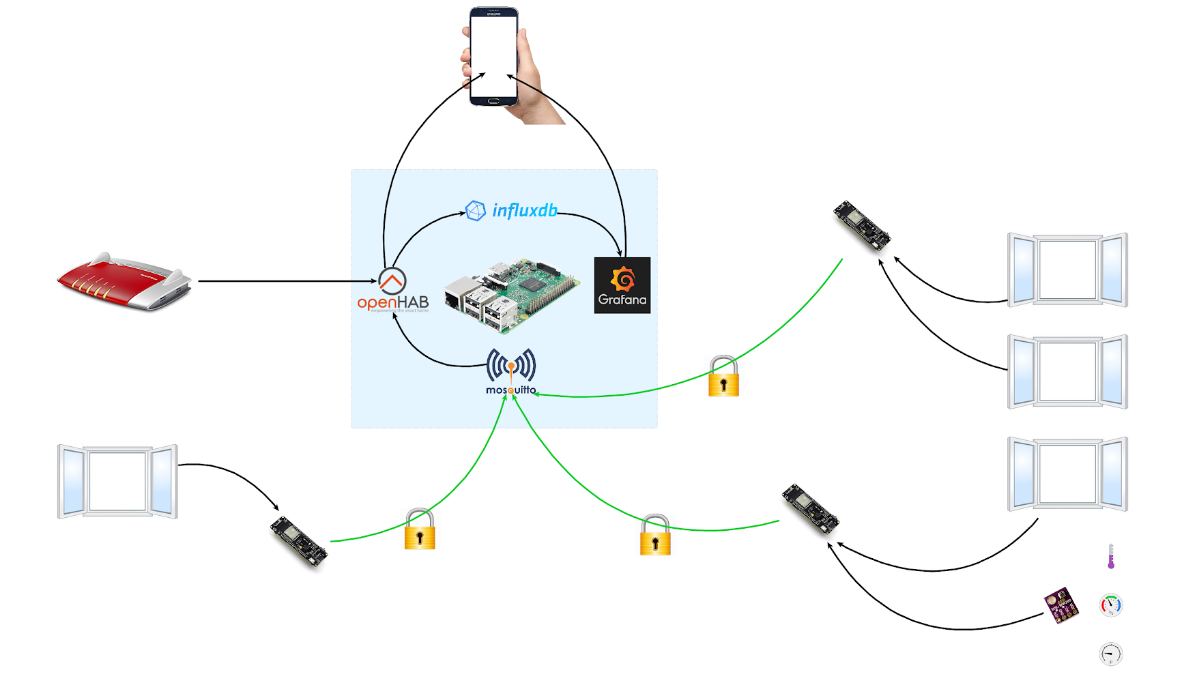
\includegraphics[width = (\textwidth)/2]{images/systemuebersicht.png}
\caption{Systemübersicht}
\label{fig:systemuebersicht}
\end{figure}\\\\
Die Anforderungen als Grundlage nehmend, ist die Ausarbeitung des Gesamtsystems und Ermittlung der zur Umsetzung nötigen Komponenten der nächste Schritt.
Folgende Aspekte werden dazu berücksichtigt:
\begin{itemize}
    \item Hardware
    \item Software
    \item Kommunikation der Systemkomponenten
    \item Datensicherung
    \item Funktionsablauf
    \item User-Schnittstelle
\end{itemize}\\\\
Das zentrale Element des Systems ist eine Smart Home Zentrale, welche mit mehreren Knoten verschlüsselt über \ac{MQTT} kommuniziert. Ein Knoten ist Schnittstelle für alle Sensoren, die zum Einsatz kommen sollen. Die Knoten senden die Messdaten über das MQTT-Protokoll an die Smart Home Zentrale, wo sie dann alle in einer Datenbank persistiert werden. Diese Messdaten werden dem User über eine Webschnittstelle angezeigt. Über diese ist ebenfalls die Aktivierung des Systems steuerbar.\\\\
Im konkreten Anwendungsfall sendet der Knoten eine  Nachricht, wenn ein Fenster geöffnet wurde, daraufhin authentifiziert der Message Bus (MQTT) den Knoten und akzeptiert die Nachricht. Die Zentrale nimmt dann die Nachricht an, verarbeitet sie und sendet eine Nachricht, wenn die Bedingungen \textit{Security aktiv} und \textit{Fenster wird geöffnet} erfüllt wurden.

\paragraph{Systemkomponenten}
\begin{itemize}
    \item Smart Home Zentrale
    \item Sensor-Knoten
    \item Sensoren
\end{itemize}

\section{Wahl der Systemkomponenten}
Zur Umsetzung des Systems in die Praxis musste nun eine Wahl getroffen werden, welche (Hardware und Software) Komponenten in der Praxis zum Einsatz kommen sollen und aus welchen Gründen. Hierzu werden mehrere alternative Lösungen gegenübergestellt und abgewägt, mit welcher Lösung sich die Anforderungen am besten und nachhaltigsten erfüllen lassen.\\
Bei der Wahl der Soft- und Hardware muss die Kompatibilität zwischen den beiden Bereichen berücksichtigt werden. Trotzdem werden im Folgenden die Komponenten der beiden Bereiche in separaten Kapiteln betrachtet.

\subsection{Hardware}

Auf der untersten Schicht des Systems ist die Hardware, auf der die zur Umsetzung des Systems nötige Software installiert wird.

Diese gliedert sich in folgende Untergebiete:
\begin{itemize}
    \item Gerät zum Einsatz als Smart Home Zentrale (1 x)
    \item Gerät zum Einsatz als Sensor-Knoten (mehrfach)
    \item Sensoren (mehrfach)
    \begin{itemize}
        \item Fenster-Sensor
        \item optional weitere Sensoren (z. B. Umweltsensor: Temperatur, Luftfeuchtigkeit, Luftdruck, Gas)
    \end{itemize}	
\end{itemize}

\subsubsection{Smart Home Zentrale Board}
Softwareseitig soll openHAB als Smart Home Sever eingesetzt werden (siehe Kapitel Software - openHAB). Im Folgenden wird die Entscheidung für die Wahl der Hardwarelösung zur Umsetzung der Smart Home Zentrale begründet. 

\paragraph{PC oder Microcontroller} OpenHAB kann auch auf einem PC laufen, jedoch muss dieser zur Aufrechterhaltung des Sicherheitssystems ständig in Betrieb sein. Einen PC eigens für diese Aufgabe einzusetzen ist nicht ressourcensparend und beinhaltet unnötig viele Funktionalitäten, welche die Kosten des gesamten Smart Home Systems (Stromverbrauch, Hardware-Anschaffung) unnötig in die Höhe treiben würden. Daher muss ein Gerät gewählt werden, welches folgenden Grundanforderungen entspricht.
\begin{itemize}
    \item unterstützt ein OS, welches die Installation von openHAB ermöglicht
    \item WLAN Modul 
    \item ein Gerät, welches eine höhere Leistungsfähigkeit bietet, um als Server für mehrere Sensor-Knoten eingesetzt zu werden
\end{itemize}\\\\
Aufgrund der allgemeinen Bekanntheit und Benutzerfreundlichkeit des \textit{Raspberry Pi}\footnote{Alle Raspberry Pi Modelle ab Version 2 sind für den Einsatz als Smart Home Zentrale zu empfehlen. Es bietet sich jedoch an, mindestens die Version 3 zu wählen, da dort ein WLAN Modul bereits fest integriert ist und nicht separat erworben werden muss.} haben wir uns dafür entschieden, diesen als Smart Home Zentrale einzusetzen.

\subsubsection{Sensor-Knoten Boards} 
Die Anforderungen an ein Sensor-Knoten Board sind die folgenden:
\begin{itemize}
    \item \textbf{WLAN (802.11n) Modul integriert:} zur Kommunikation über größere Entfernungen; zur Verbindung mehrerer Geräte mit der Smart Home Zentrale (bei Bluetooth gibt es eine Beschränkung bis 8 Geräte); daher nicht Bluetooth
    \item \textbf{Große User-Community:} große, internationale Bekanntheit des Boards; Durch eine große User-Community kann man von der Erfahrung vieler Nutzer profitieren. Es stehen viele Erfahrungsberichte und Tutorials (frei) zur Verfügung.
    \item \textbf{Günstiger Preis:} Mehrere Boards können gekauft werden, wenn der Bedarf (z. B. bei vielen Fenstern in einem Haus) besteht
    \item \textbf{Programmierbare Hardware:} Nutzer sind nicht an eine Technologie gebunden, sondern können ein eigenes System ausarbeiten und ausführen.
    \item \textbf{Akku-Betrieb:} Keine kabelgebundene Stromversorgung mit dem Zwang, Kabel verlegen zu müssen notwendig
    \item \textbf{Stromsparend:} die Boards sollen so lange wie möglich ohne Wiederaufladung der Akkus betrieben werden
    \item \textbf{Platzsparend, möglichst kleine Abmessungen:} Da dieses Gerät am oder in der Nähe eines Fensters platziert werden soll, ist es wünschenswert, dass es optisch nicht zu stark auffällt.
\end{itemize}\\\\
Der Mikrocontroller \textit{ESP32} der chinesischen Firma \textit{Espressif Systems}\footnote{\url{https://www.espressif.com}} hat am besten den oben genannten Anforderungen entsprochen und wurde daher für den Einsatz als Sensor-Knoten ausgewählt.
\paragraph{Hardwaremerkmale des ESP32 Boards} 4 MB Flash, Dual Core, Ladetechnik und 18650 Akku Anschluss, Eingebaute Funkmodule (WLAN + Bluetooth)
\paragraph{Vorteile gegenüber anderen Board Alternativen} Im Vergleich zu anderen Boards, die \textit{RIOT OS} als Betriebssystem unterstützen\footnote{Unterstützung von RIOT OS für ESP32 Boards ist bereits in der Entwicklung und soll noch folgen: \url{https://github.com/gschorcht/RIOT-Xtensa-ESP/wiki}}, sind ESP32 Boards \textbf{kostengünstig} erhältlich, was bedeutet, dass es eine \textbf{große User-Community} gibt, sodass viele Tutorials und eine ausführliche Dokumentation der Hardwarefunktonalität zur Verfügung stehen, welche die Einarbeitung in die Handhabung des ESP32 erheblich erleichtern.\\
Bei möglichen Alternativen zum ESP32 Board\footnote{Alternativen zum ESP32: z. B. der Vorgänger ESP8266; weitere Alternativen: \url{https://github.com/RIOT-OS/RIOT/tree/master/boards}}, die RIOT OS unterstützen würden, wird die Entwicklung und damit der Support eingestellt, was für die Entwicklung eines zukunftsorientierten Systems nicht annehmbar ist. 

\begin{itemize}
    \item geringer Preis
    \item große User-Community
    \item low-power Mikrocontroller
\end{itemize}
Der Vorgänger des ESP32, ESP8266 (von Espressif Systems) ist ebenfalls weit verbreitet, ihm fehlen jedoch folgende Eigenschaften, die für unser System von Nutzen sind: 

\begin{itemize}
    \item Verschlüsselungskoprozessor
    \item bessere Antenne
    \item mehr Speicher
    \item Deep Sleep mit 5 $\mu A$ Stromverbrauch\footnote{Nur der Chip allein, ohne Peripherie}
\end{itemize}

\paragraph{Wahl des Betriebssystems} Aus den oben genannten Kosten- und Kompatibilitätsgründen wurde für dieses Projekt nicht RIOT OS eingesetzt. Stattdessen wird \textit{FreeRT OS}\footnote{FreeRTOS: https://www.freertos.org/} eingesetzt, das von Espressif zur gemeinsamen Benutzung mit \ac{ESP-IDF} empfohlen wird.\footnote{https://esp-idf.readthedocs.io/en/v2.0/build-system.html}
Die Wahl des Betriebssystems folgte der weiten Verbreitung und der großen Entwicklergemeinschaft. Wir wollen auch in Zukunft Patches ausliefern können und da ist ein weit verbreitetes Betriebssystem ideal. Zusammen mit der \ac{ESP-IDF} gibt es den Arduino Core\footnote{\url{https://github.com/espressif/arduino-esp32}} für den ESP32. Durch Verwendung dieser Bibliothek ist es möglich, Arduino-kompatiblen Code zu schreiben, der auch auf anderen von Arduino unterstützten Geräten benutzt werden kann. Lediglich native Aufrufe, wie es beispielsweise beim Aufruf des Deep Sleep der Fall ist, müssten angepasst werden. Ein weiterer Vorteil neben der erhöhten Portabilität ist die Tatsache, dass man alle für Arduino entwickelten Dritt-Bibliotheken einbinden und nutzen kann. So können wir z.B. auch die MQTT Implementierung \textit{arduino-mqtt}\footnote{\url{https://github.com/256dpi/arduino-mqtt}} nutzen.

\subsubsection{Sensoren} 
Die Boards sind relativ leistungsstark und unterstützen diverse Sensoren. Wir haben für unseren Use-Case Magnetsensoren für Türen und Fenster integriert, welche lediglich einen Stromkreis öffnen und schließen. Es können bis zu 2 Sensoren pro Knoten angeschlossen werden. Für eine mögliche Erweiterung des Systems wurden auch Umgebungssensoren (Temperatur/ Luftdruck/ Luftfeuchtigkeit) integriert. So können wir die Raumluft überwachen und das System mit zusätzlichen Information interessanter gestalten. Wir unterstützen die Bosch Sensoren BME280\footnote{\url{https://www.bosch-sensortec.com/bst/products/all\_products/bme280}} und BME680\footnote{\url{https://www.bosch-sensortec.com/bst/products/all\_products/bme680}}. Die Wahl fiel auf diese Sensoren, da die Qualität gegenüber den fast gleich teueren DHT22 wesentlich besser ist.
(siehe Abb. \ref{fig:temparatur_sensoren_vergleich}, S. \pageref{fig:temparatur_sensoren_vergleich})
 
\begin{figure}[htb!]
\centering
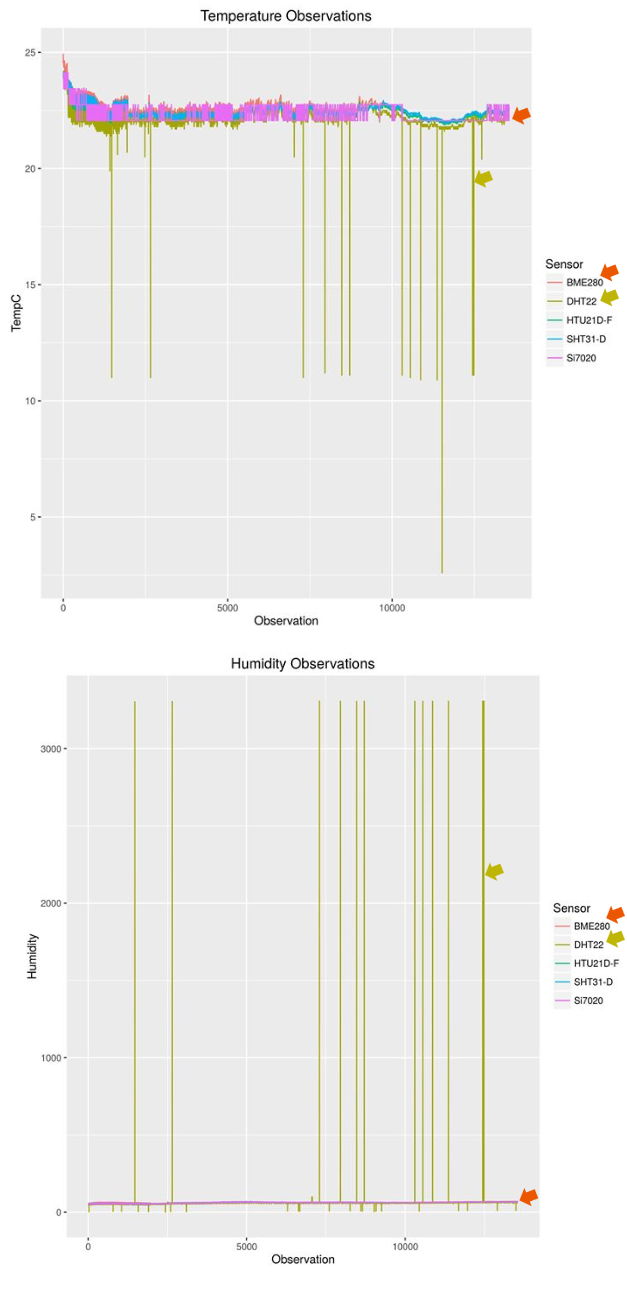
\includegraphics[width = (\textwidth)/2]{images/temparaturSensoren_vergleichV.png}
\caption[Vergleich der Stabilität der Messwerte für die Sensoren BME280, DHT22, HTU21D-F, SHT31-D, Si7020]{Vergleich der Stabilität der Messwerte (Temperatur und Luftfeuchtigkeit) für die Sensoren BME280, DHT22, HTU21D-F, SHT31-D, Si7020; Der gewählte BME280 gehört zu den Sensoren mit einer guten Messstabilität, im Vergleich dazu treten beim DHT22 häufig starke Schwankungen in der Messgenauigkeit auf.}
\label{fig:temparatur_sensoren_vergleich}
\end{figure}


\subsection{Kommunikationsmechanismus}
\subsubsection{(Drahtlose) Kommunikationstechnologie}
Für dieses Projekt standen mehrere Funkstandards zur Verfügung. Die drei am besten geeigneten sind:
\begin{description}
\item[802.11 (Wifi)] 
ist ein sehr beliebter Funkstandard und in nahezu jedem modernen Zuhause bereits verfügbar.\footnote{Bei SmartHome interessierten setzen wir ein verfügbares WLAN voraus.} Die moderneren Standards ermöglichen einen sehr hohen Datensatz, aber der Funkstandard ist nicht sehr energieeffizient. Ein WLAN-Netzwerk kann sehr viele Geräte verwalten.
\item[802.15.1 (Bluetooth)]
ist ein Nahfeldfunkstandard. Er wurde entwickelt um Daten zwischen Geräten in kurzer Distanz zu übertragen. Die Reichweite der meisten verfügbaren Geräte beträgt circa 10 Meter und seit Version 4.0 gibt es einen Energiesparmodus, der den Stromverbrauch deutlich reduzieren kann. Es lassen sich bei vielen Geräten nicht beliebig viele pairen (verbinden) und erst mit Version 5.0 können zwei Verbindungen gleichzeitig gehalten werden.
\item[802.15.4 (6LoWPAN)]
ist ein Funkstandard, der speziell für stromsparende Netzwerke erstellt wurde und wird bei IoT Projekten gerne verwendet. Er erfüllt alle Kriterien, die wir an ihn stellen. Lediglich die Auswahl der Mikrocontroller ist begrenzt und erfüllt unsere Erwartungen momentan nicht.
\end{description}

Bluetooth ist schnell aus unserer Betrachtung gefallen, weil wir keine Geräte mit Protokollversion 5 günstig erwerben konnten und auch die Erweiterbarkeit des Netzwerkes schien uns zu aufwendig für unser Projekt\footnote{Wir wollen eine Installation leicht machen und wenn wir eigene Repeater oder Access Points bauen müssen, wäre das zu umfangreich geworden.}. Zudem spricht die verfügbare Reichweite gegen Bluetooth. Für WLAN spricht die weite Verfügbarkeit und einfache Erweiterung des Netzwerkes mit Repeatern etc. Es ist sogar recht Preiswert alle Smart-Home Geräte über ein seperates Funknetzwerk komplett vom Rest abzukapseln. Was den Zuspruch für WLAN brachte waren die niedrigpreisigen und weit verfügbaren Mikrokontroller. Die Kosten des Projekts auf Basis von 6LoWPAN Kommunikation würden derzeit zu hoch sein. Durch die gängigen Kommunikationsprotokolle sollte es aber kein Problem sein, in Zukunft auch solche Geräte einbinden zu können, wenn man einen Access Point in das System integriert.

\subsubsection{Kommunikationsprotokolle}

Wir haben uns beim Übertragen der Daten vom Mikrokontroller zu der Smarthome-Zentrale für \ac{MQTT} entschieden. \ac{MQTT} steht für "Message Queue Telemetry Transport" und ist ein offenes Nachrichtenprotokoll für Machine-to-Machine-Communication (M2M). Dabei schreiben die Knoten ihre Nachrichten in ein Topic, das von der SmartHome-Zentrale abbonniert wird. Es konsumiert die Nachrichten und reagiert entsprechend darauf. Der Vorteil, den das Protokoll bietet ist, dass die Nachrichten asynchron und mit Störungen klarkommt, sodass die Nachrichten ggf. nochmals gesendet werden. Zuverlässigkeit ist für eine Sicherheitsanwendung essentiell.\\\\
Als Broker haben wir uns für Mosquitto entschieden, da die Software Open Source und sehr leichtgewichtig ist. Sie läuft problemlos parallel auf einem Raspberry Pi mit openHAB und allen anderen genutzten Diensten zusammen.\\\\
Die Topics können frei gewählt werden, wobei wir uns für folgendes Muster entschieden haben:
\begin{lstlisting}[numbers=none]
room/office/nodeID/WindowSensor1
room/livingroom/nodeID/humidity
\end{lstlisting}\\\\
Zu Beginn beschreiben wir die Wohneinheit. Derzeit gibt es nur Räume, aber eine Erweiterung auf den Garten oder Haus (Gesamtstromverbrauch des Hauses etc.) ist denkbar. Als nächste Einheit wird der Raum näher spezifiziert. Danach folgt eine Knoten-ID zur Identifizierung des Knotens und dann die einzelnen Sensoren, die angeschlossen wurden.

\subsection{Software}

\subsubsection{Smart Home Zentrale}

Die Smart Home Zentrale stellt die zentrale Komponente in unserem Projekt dar. Sie führt alle Sensordaten zusammen, speichert deren Verläufe, sendet Benachrichtigungen und bereitet die Daten für die Nutzer grafisch auf. Sie muss erweiterbar sein und sich in das bestehende Smart Home integrieren. Nicht zu vergessen, es ist für uns wichtig, dass die Zentrale mit Open Source Software mit Standardprotokollen läuft, damit wir das System in Zukunft warten und austauschen können. Der vielversprechendste und eingesetzte Kandidat ist \acf{openHAB}.\\\\
OpenHAB wird seit Jahren von der Eclipse Foundation entwickelt. Sie ist sehr finanzkräftig und die große Nutzercommunity lässt uns hoffen, dass das System noch mehrere Jahre entwickelt und gewartet wird. Es wurde in Java geschrieben und läuft daher auf allen gängigen Plattformen, ganz egal ob auf einem Server, Notebook oder Raspberry Pi. Für unsere Tests haben wir verschiedene Varianten des Raspberry Pi (2b,3b und 3b+) verwendet. Sie dienten als untere Leistungsschranke, für die wir das System optimieren wollten. Außerdem wird ein fertiges Image auf Raspbian-Basis von openHAB bereitgestellt, was uns für eine vereinfachte Bedienung entgegenkommt.\\\\
OpenHAB hat eine Plugin Architektur, was es erlaubt verschiedene Systeme und Technologien anzubinden. Derzeit sind es über 200 inklusive den Marktführern wie Philips Hue. Es können Befehle gesendet und empfangen werden, um somit Aktionen zu steuern. Dies ist ein wichtiger Punkt. Das Installieren der Bindings über die Webschnittstelle ist sehr komfortabel. Wir haben das MQTT, Influx, OpenHAB-CloudConnector und das Fritzbox TR064 Binding verwendet.

\begin{itemize}
    \item MQTT Binding erlaubt uns die Sensordaten von MQTT auszulesen und zu benutzen.
    \item Influx Binding persistiert die Sensordaten für Grafana für die späteren Auswertungen.
    \item OpenHAB-CloudConnector lässt uns die Verbindung zu myopenhab.org aufbauen, damit wir Push-Notifications auf unsere Smartphones senden lassen können.
    \item Fritzbox TR064 Binding ist optional und erlaubt es uns das Sicherheitssystem automatisch zu aktivieren, wenn die Besitzer mit dem Smartphone das Haus verlassen.
\end{itemize}

\paragraph{Wie haben wir unsere Sensoren integriert?} Dazu haben wir für openHAB Items angelegt. Ein Item hat einen Typ und einen Zustand. Es kann ein Schalter sein, der An oder Aus ist oder eine Temperaturanzeige, welche die Raumtemperatur zeigt. Zum Anlegen neuer Items editiert man eine Konfigurationsdatei auf dem Server, indem man den Typ, Namen, Icon, Gruppe und die Binding-Konfiguration angibt. In unseren Fall war die Binding-Konfiguration das \ac{MQTT}-Topic, an welches die Knoten senden. Anschließend lädt openHAB die Konfiguration sofort neu und das Item ist dem System von da an bekannt.

\begin{figure}[htb!]
\centering
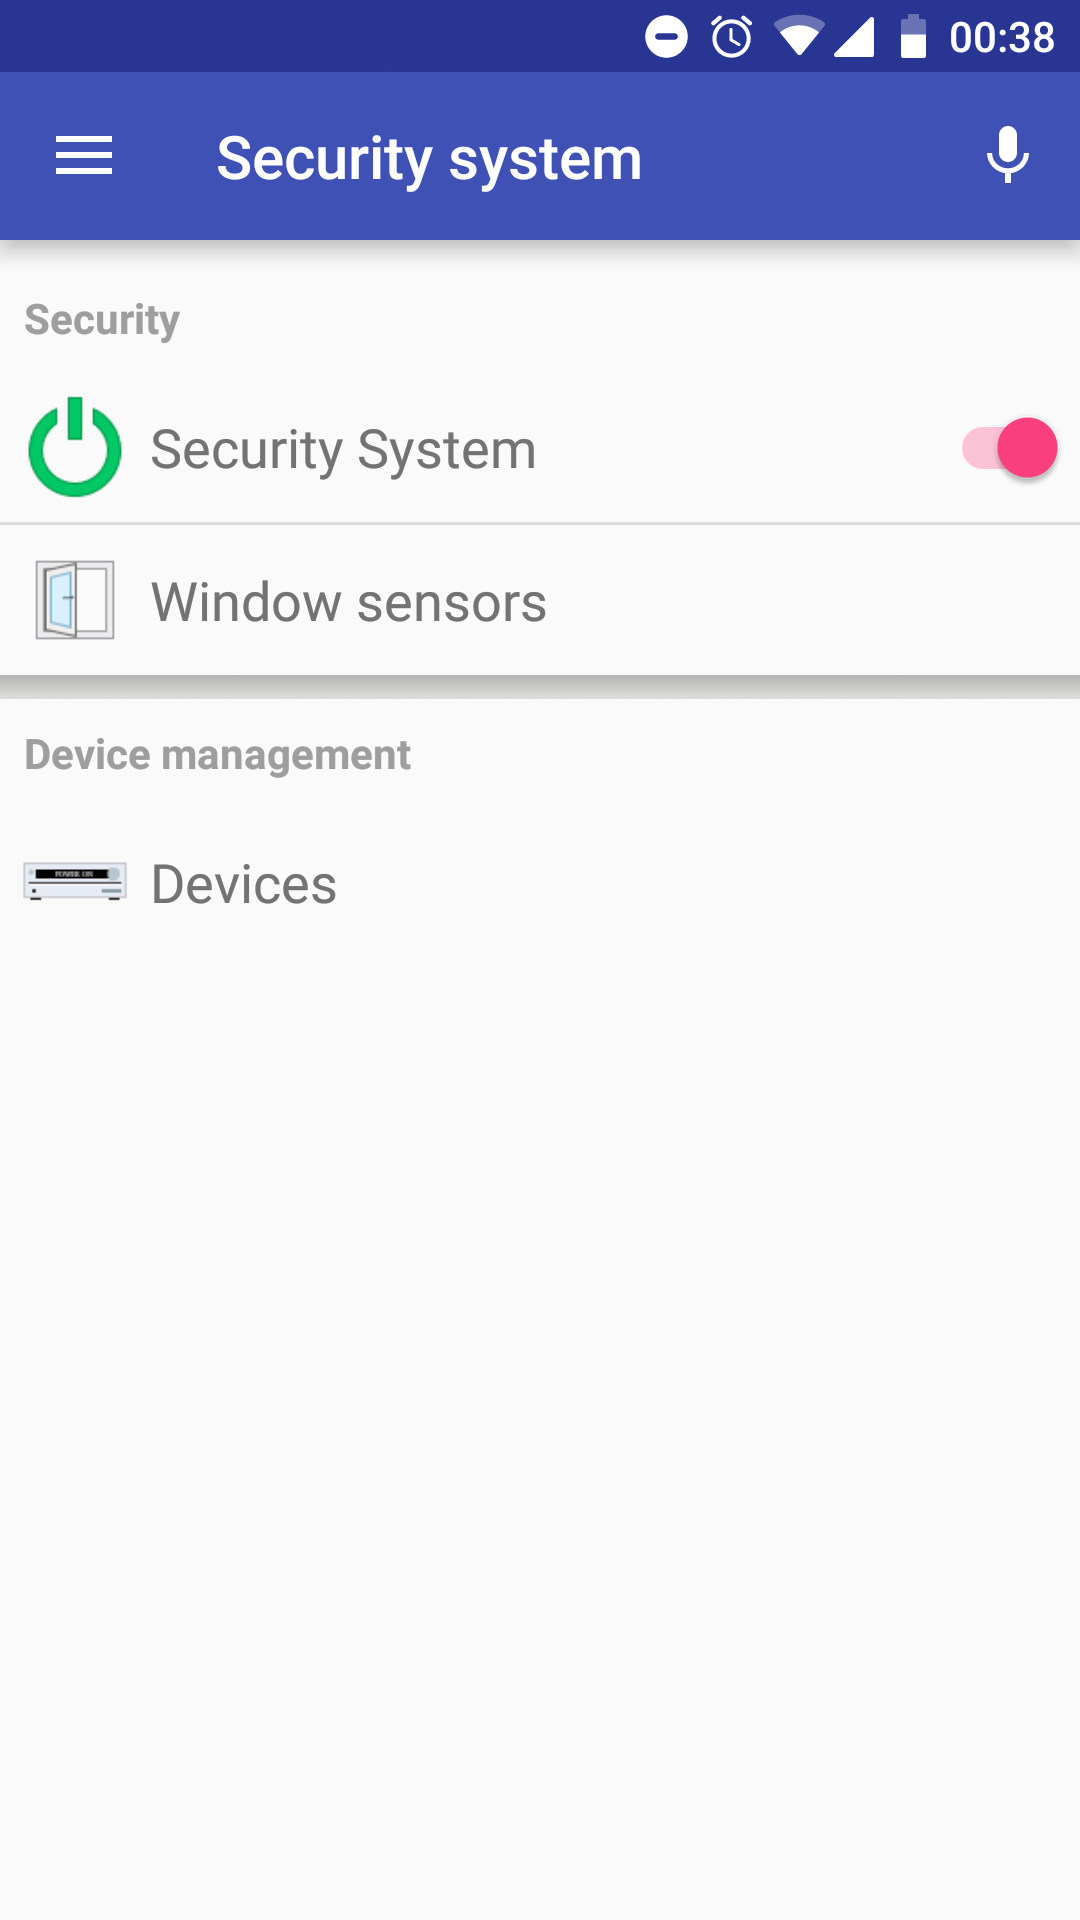
\includegraphics[width = (\textwidth)/3]{images/openhab_app.png}
\caption{openHAB User-Schnittstelle über die Smartphone App}
\label{fig:openhab_app}
\end{figure}

\paragraph{User-Schnittstelle}
Nutzer haben auf verschiedene Weise Zugriff auf die Smart Home Daten. Zum Einen gibt es folgende Möglichkeiten auf openHAB zuzugreifen: 
\begin{itemize}
    \item über die openHAB App auf dem Smartphone (siehe Abb. \ref{fig:openhab_app}, S. \pageref{fig:openhab_app}) oder der Smart Watch
    \item über das Web-Interface von openHAB (erreichbar (beim Einsatz eines Raspberry Pi) über \texttt{openhabianpi:8080})
\end{itemize}\\\\
OpenHAB kann so eingestellt werden, dass es die Sensordaten in InfluxDB persistieren, also speichern soll. So können ggf. die Änderungen am System nachverfolgt und Alarme ausgeben werden, falls eine längere Zeit keine Daten mehr kommen. Die Aufbereitung der Daten übernimmt Grafana, welches ein Analyse- und Monitoring-Werkzeug ist (siehe Abb. \ref{fig:grafana}, S. \pageref{fig:grafana}).\\\\
OpenHAB liest aus MQTT alle Sensordaten, stellt sie in der GUI dar, löst Alarme aus und speichert die Daten in einer Datenbank, aus welcher Grafana Graphen über den Verlauf erstellt und ebenfalls Warnungen erstellt, falls Daten ausbleiben.\\\\
All diese Funktionen und der \ac{MQTT}-Broker laufen auf einem Raspberry Pi ohne die Ressourcen übermäßig zu beanspruchen. Deswegen rechnen wir nicht mit Problemen im Dauerbetrieb mit den Geräten.

\begin{figure}[htb!]
\centering
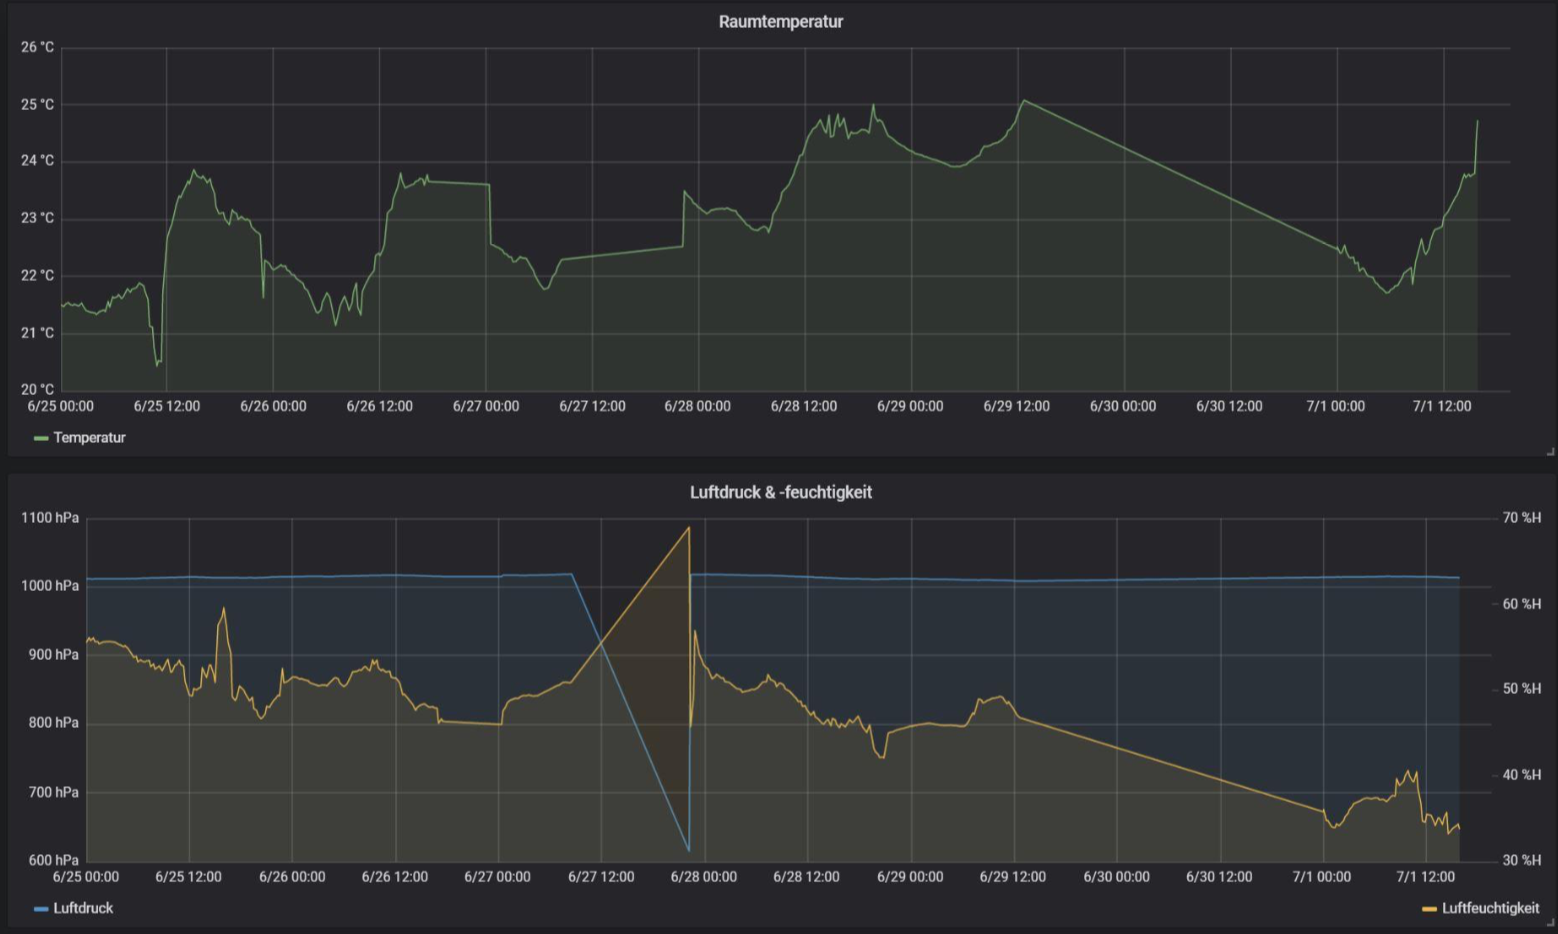
\includegraphics[width = (\textwidth)/2]{images/grafana.png}
\caption{Grafische Darstellung der Sensormesswerte in Grafana}
\label{fig:grafana}
\end{figure}

\section{Umsetzung}

\subsection{Sicherheitsmerkmale}
\subsubsection{Angriffserkennung}
\paragraph{Akustisches Signal} Mithilfe des Anschlusses eines Lautsprechers an die Smart Home Zentrale kann, sobald ein Alarm ausgelöst wird, ein Signalton abgespielt werden. Dieser kann nur wieder über die Webschnittstelle von openHAB deaktiviert werden.

\paragraph{Störung des Funkkanals} Die Smart Home Zentrale (Raspberry Pi 3/3+) hat ein WLAN-Modul. Dieses überprüft per Cron-Job die WLAN-Qualität. Sobald die Qualität des WLAN unter einen festgelegten Schwellenwert fällt, wird in der Standardkonfiguration ein stiller Alarm ausgelöst. Das bedeutet, dass der Nutzer zwar eine Benachrichtigung über das schlechte WLAN-Signal erhält, allerdings kein akustischer Alarm ausgelöst wird. Ansonsten könnte es unter Umständen zu einer Vielzahl an Fehlalarmen führen. Der Server sollte für den tatsächlichen Betrieb über LAN an den Router angeschlossen sein, sodass er im Falle einer Funkstörung weiterhin von außen erreichbar ist und auch die Benachrichtigung über den Alarm an den Nutzer absetzen kann.

\subsubsection{Lost Node Detection}
Da wir durch Stromsparmaßnahmen die Knoten nicht von der Zentrale aus ansprechen können, können wir nur das Fehlen von Nachrichten als ausgefallenen Knoten betrachten. Deswegen wird die Eigenschaft unserer Anwendung ausgenutzt, dass jeder Knoten in einem konfigurierten Zeitintervall eine Nachricht mit den aktuellen Sensordaten sendet. Da alle Änderungen in Influx persistiert werden, kann Grafana dem Nutzer Benachrichtigungen über fehlende Nachrichten von einzelnen Knoten zusenden. Grafana unterstützt verschiedene Benachrichtigungsformen, getestet haben wir die Benachrichtigung in Form einer Email.\\
Grafana bietet einen Webhook an, der anstatt oder zusätzlich zu einer Email benutzt werden kann. Wir wollten dies mit der Rest-API von openHAB verbinden, was allerdings nicht gelang, weil der Webhook den Mediatype nicht mitsendet und openHAB dabei wenig tolerant ist. So müssen wir mehrere Benachrichtungskanäle einrichten, anstatt alles über die Push-Notifications von openHAB laufen zu lassen.

\subsubsection{Physischer Zugriffsschutz}
Zusätzlich neben dem Schutz der Kommunikationskanäle, den verschiedenen Servern und deren dort gespeicherten Daten können auch die Knoten selbst vor physischem Zugriff geschützt werden. Espressif hat dazu in den ESP32 Unterstützung für Flash Encryption\cite{ESPFlashEncryption} und Secure Boot\cite{ESPSecureBoot} implementiert. Mithilfe von Flash Encryption ist es beispielsweise nicht mehr möglich, in dem Chip abgespeicherte Daten wie etwa das WLAN-Passwort auszulesen. Durch Secure Boot wird verhindert, dass andere Programme auf dem Chip installiert werden, die keine korrekte Signatur aufweisen.\\\\
Da es sich bei diesem System um ein Alarmsystem für ein Haus oder eine Wohnung handelt, haben wir aufgrund der Tatsache, dass bei einem physischen Zugriff auf das Gerät im Haus durch Dritte bereits andere Probleme bestehen, diese Möglichkeiten nicht weiter erforscht. In anderen Anwendungen, wo das Gerät öffentlich zugänglich ist, ist eine Verwendung dieser Funktionen sinnvoller.

\subsubsection{Mesh Netzwerk}
Durch Verwendung eines Mesh-Netzwerkes können die Daten eines Geräts über mehrere andere Geräte hinweg weitergeleitet werden, ehe sie ihr Ziel erreichen. Einer der größten Vorteil eines solchen Netzwerkes ist die verbesserte Reichweite, die ansonsten nur mit größerer Infrastruktur, wie etwa Einsatz von WLAN-Repeatern, erreicht werden könnte. Ebenfalls von Vorteil ist es, dass das Netzwerk eben nicht auf besagte Repeater angewiesen ist. Sollte ein Repeater ausfallen, so wären unter Umständen mehrere Knoten vom Netzwerk getrennt. Sollte bei einem Mesh-Netzwerk ein Knoten ausfallen, könnte sich die Netzwerkstruktur neu aufbauen und anpassen, sodass die übrigen Knoten weiterhin alle erreichbar sind, was die Ausfallsicherheit der einzelnen Knoten erhöht.\\\\
Wir haben uns gegen eine Nutzung entschieden, da ein derartiges Netzwerk aus unserer Sicht nicht mit unseren Stromsparzielen (Kap. \ref{sec:stromsparmassnahmen}, S. \pageref{sec:stromsparmassnahmen}), welche einen hohen Stellenwert in den Anforderungen einnehmen, zu vereinbaren ist. Eine eventuell angestrebte Reichweitenverbesserung des Netzwerkes kann stattdessen durch den Einsatz von WLAN Repeatern erreicht werden.

\subsubsection{Absicherung der Kommunikation über Mosquitto}
Eine Absicherung der Kommunikation über Mosquitto ist essentiell, da der Transport der Nachrichten über den Fensterstatus sicherheitskritisch ist.\\
Dazu wird \ac{TLS} im Mosquitto \ac{MQTT} Broker eingerichtet, wobei die Smart Home Zentrale als \ac{CA} dient. Eine sichere Authentifikation wird über Client Zertifikate realisiert. Die Ausstellung dieser ist ebenfalls Aufgabe der \ac{CA}.

\subsection{Stromverbrauch}
Die ESP32 Boards haben eine Akkuhalterung, wodurch die Boards mit Lithium-Ionen vom Typ 18650 betrieben werden können.\\
Das Laden der Akkus über das Board ist möglich, sodass die Akkus nicht zwangsläufig herausgenommen und über ein externes Ladegerät wieder aufgeladen werden müssen.

\subsubsection{Stromsparmaßnahmen}\label{sec:stromsparmassnahmen} 
\paragraph{Schlafmodus} Die Idee hinter dem Schlafmodus ist es, das Board nur dann wirklich aktiv zu betreiben, wenn tatsächlich Arbeit anfällt. Dazu können entweder der Light Sleep oder der Deep Sleep verwendet werden, die vom ESP32 hardwareseitig unterstützt werden. Aktiv ist das Gerät nur nach folgenden Ereignissen
\begin{itemize}
    \item Weckruf nach einem Intervall, bei dem Sensordaten übermittelt werden sollen
    \item Interrupt nachdem ein Fenster geöffnet oder geschlossen wurde
\end{itemize}
Der \textit{Deep Sleep} \cite{ESPDeepSleep} führt im Gegensatz zum Light Sleep zum Reset des ESP32. Das bedeutet, dass nach dem Aufwachen alle Prozeduren neu ausgeführt werden müssen, unter anderem also auch Verbindungen neu hergestellt werden müssen. Der ebenfalls verfügbare \textit{Light Sleep} \cite{ESPSleepModes} ist hingegen weitaus schneller, da die CPU die Ausführung dort fortsetzt, wo der Light Sleep initiiert worden ist. Nachteil hierbei ist der erhöhte Stromverbrauch, da der Ausführungszustand im \ac{RAM} gespeichert werden muss. Beim Light Sleep muss beispielsweise der \ac{RAM} also zwangsläufig weiterhin mit Strom versorgt werden, während dieser beim Deep Sleep abgeschaltet werden kann.\\
Um den Chip wieder aufzuwecken gibt es verschiedene Möglichkeiten. Entsprechend der oben genannten Ereignisse wird ein Timer-Interrupt benötigt. Hierfür wird die integrierte RTC im ESP32 verwendet. Für externe Interrupts, die für die Fenstersensoren benötigt werden, stehen 2 Quellen zur Verfügung: \textit{ext0} und \textit{ext1}. Die beiden Quellen unterscheiden sich stark. An \textit{ext0} kann immer nur ein einziger GPIO Pin gleichzeitig gebunden werden. Ein einzelner Fenstersensor belegt damit bereits den ersten externen Interrupt. An die zweite Quelle \textit{ext1} können zwar mehrere GPIO Pins gebunden werden, allerdings werden diese untereinander in einem analogen Logikgatter verbunden. Die möglichen Konfigurationen von \textit{ext1} sind entweder \textit{ANY\_HIGH} oder \textit{ALL\_LOW}. Während \textit{ANY\_HIGH} unproblematisch ist, beschränkt \textit{ALL\_LOW} die Verwendung von \textit{ext1} wieder auf einen einzigen Fenstersensor. Würden mehrere Fenstersensoren an \textit{ext1} angebunden werden, müssten alle angebundenen Fenster geöffnet werden, bevor der Chip aufgeweckt wird. Das ist offensichtlich nicht praktikabel, daher ist mit dieser Architektur lediglich die Verwendung von 2 Fenstersensoren pro Gerät möglich.
\paragraph{Anwendungslogik} Weiterhin ist es möglich mit erweiterter Anwendungslogik noch mehr Strom zu sparen, z.B. indem der Grund für das Aufwecken betrachtet wird. So besteht beispielsweise nicht bei jedem Öffnen des Fensters die Notwendigkeit nach einer möglichen Aktualisierung zu suchen. Glücklicherweise lässt sich der Grund für das Aufwecken des ESP32 auslesen, jedoch nur für den Deep Sleep. Für den Light Sleep scheint die entsprechende Methode nicht geeignet zu sein. Wird ein Fenster geöffnet, wird lediglich der Fensterstatus an die Zentrale gesendet. Wird das Gerät allerdings durch den Timer aufgeweckt, so werden sowohl der Fensterstatus, als auch die Daten des Umgebungssensors übermittelt. Außerdem findet eine Prüfung nach einer eventuellen Aktualisierung statt.
\paragraph{Konfiguration} Ebenfalls möglich sind weitere Energieeinsparungen mittels der Konfiguration des ESP32. Dort sollte der zweite CPU-Kern deaktiviert werden, da dieser für unsere Anwendung nicht benötigt wird. Eine Senkung der Taktfrequenz ist nicht zu empfehlen, da dadurch die Latenz bis zum Alarm erhöht wird. Zwischen der niedrigsten (80 MHz) und der höchsten (240 MHz) Taktfrequenz macht das im Durchschnitt etwa 4.5 Sekunden Unterschied\footnote{siehe Messungen im Repository\cite{smarthome2} unter misc/measurements/runtimes/} aus.
\paragraph{Deaktivierung von Funktionalität} Es ist davon auszugehen, dass durch Verzicht auf die implementierten Sicherheitsmaßnahmen messbar Strom eingespart werden könnte. Liegt der Fokus ausschließlich auf dem Alarmsystem, könnte ebenfalls auf zusätzliche Sensorik verzichtet werden. Im Zuge dessen könnte auch auf den Intervall-Weckruf verzichtet werden, wenn kein \ac{OTA}-Update bereitgestellt werden soll. Dann würde der Knoten nur noch beim Öffnen und Schließen von Fenstern aufgeweckt werden.

\subsubsection{Akkulaufzeit}
Das erklärte Ziel in den Anforderungen ist, dass die verbauten Lithium-Ionen Akkus vom Typ 18650 \textit{mindestens ein Jahr} ohne erneutes nachladen genutzt werden können. Für genauere Werte wird zwar ein langer Testzeitraum benötigt, jedoch kann die Laufzeit mithilfe der erstellten Rechentabelle\footnote{Im Repository\cite{smarthome2}: \mbox{misc/power\_consumption\_calculation.ods}} abgeschätzt werden.\\\\
Zur Berechnung von Beispiellaufzeiten wird die folgende Konfiguration angenommen:
\begin{itemize}[noitemsep]
    \item Stromverbrauch aktiv: 120 mA
    \item Stromverbrauch im Deep Sleep: 55 $\mu A$
    \item Akkukapazität: 3400 mAh
    \item Aktive Zeit pro Weckruf: 9 s
    \item Selbstentladung von 4\% pro Monat \cite[S. 20]{umweltbundesamt}
\end{itemize}
In der folgenden Tabelle ist das Weckintervall variabel, da es der treibende Faktor für den Stromverbrauch ist. Vernachlässigt wird in der Berechnung die Tatsache, dass das mit dem Akku betriebene Gerät schon vor vollständiger Entladung des Akkus nicht mehr arbeiten wird, da eine Betriebsspannung von mindestens 3.3 V gehalten werden muss und die anliegende Spannung im Laufe der Entladung abfällt.\\\\
\begin{tabularx}{\textwidth/2}{lcX}
& & Akkulaufzeit\\
Aufwecken alle 15 Minuten & : & 99 Tage\\
Aufwecken alle 60 Minuten & : & 262 Tage\\
Aufwecken zweimal pro Tag & : & 532 Tage\\
\end{tabularx}\\\\
Unter Einberechnung der Selbstentladung und der zusätzlichen Beanspruchung des Akkus durch das Weckintervall zur Sensormessung sowie manuelles Fenster öffnen ist eine Akkulaufzeit von mindestens einem Jahr leider nicht realistisch. Wenn man allerdings einen zweiten Akku hinzunimmt und diese zur Kapazitätssteigerung auf 6800 mAh parallel schaltet, erzielt man bei gleichen Bedingungen bei einem Weckintervall von 60 Minuten eine Laufzeit von 389 Tagen. Dieses Ergebnis genügt uns vorerst.

\subsection{Usability} 
\subsubsection{Over-the-Air (OTA) Updates}
Sind die einzelnen Geräte erst montiert, ist es von Vorteil einen Mechanismus anzubieten, der es ermöglicht, Updates leicht durchführen zu können, ohne sie wieder abbauen zu müssen. \ac{OTA}-Updates kommen daher zum Einsatz.\\\\
Nginx wird als \ac{HTTP}-Server betrieben. Eine Aktualisierung wird mittels simpler \ac{HTTP}-GET-Requests auf die auf dem Server liegenden Binärdateien abgefragt. Die URL für die Abfrage eines Boards mit der Geräte-ID \textit{esp32-1} und einer laufenden Anwendung auf Versionscode 2 lautet beispielsweise \mbox{\textit{https://local\_ota\_server/esp32-1/3/app.bin}}. Über dieses Verfahren aktualisiert sich die Version n immer zuerst auf n+1, bevor sie sich auf n+2 aktualisiert. Wird keine solche Datei gefunden, gibt der Webserver \ac{HTTP} 404\footnote{Datei nicht gefunden} zurück womit das Gerät implizit annimmt, dass es bereits mit der aktuellsten Version betrieben wird. In der Praxis sollte dies keine großen Nachteile haben, da eine Aktualisierung bei jedem Timer-Interrupt abgefragt wird und die Geräte somit im Rahmen des Weckintervalls stets aktuell sein sollten. In der Zukunft besteht hier trotzdem Optimierungsbedarf, da mit diesem Verfahren beispielsweise kein Versionscode ausgelassen werden darf.\\\\
Die Sicherheit des Updateprozesses ist besonders wichtig. Ein Aspekt ist der Schutz der Binärdateien auf dem Server selbst. In den Binärdateien sind alle Konfigurationen enthalten, welche das Gerät für den Betrieb benötigt. Dies umfasst auch sensible Daten wie das Passwort für das Heimnetzwerk und Client-Zertifikate zur Authentifikation des Gerätes am \ac{MQTT}-Broker. Eingesetzt werden deshalb, wie beim \ac{MQTT}-Broker, Client-Zertifikate, um sich gegenüber dem Webserver zu authentifizieren. Ohne entsprechende Authentifizierung wird der \ac{OTA}-Server lediglich eine Fehlermeldung zurückgeben. Weiterhin ist ein Passwort für den Zugriff auf die Binärdateien erforderlich. Ein anderer Aspekt ist der Schutz der Übertragung der Binärdateien. Um ein Abfangen der Daten während der Übermittlung zu verhindern werden die Daten ausschließlich über \ac{HTTPS} übertragen. Der ganze Prozess läuft zudem innerhalb des Heimnetzwerkes ab und ist dadurch noch stärker geschützt, vorausgesetzt der Nutzer hat dieses mit einem geheimen Passwort und starker Verschlüsselung abgesichert.

\subsubsection{Einfache und schnelle Einrichtung}
Für die Einrichtung des Systems sind zwei Komponenten zu betrachten. Einerseits die Smart Home Zentrale, andererseits die einzelnen Knoten.\\
Die Smart Home Zentrale samt all ihrer Unterkomponenten wird mithilfe von Fabric eingerichtet und verwaltet \footnote{Im Repository\cite{smarthome2}: \mbox{openHABian/setup\_openhab\_pi.py}}. Fabric ist eine Python Bibliothek, mit deren Hilfe Kommandos über SSH auf einem anderen Computer, in diesem Fall der Smart Home Zentrale, ausgeführt werden können. Auch Up- und Downloads von Dateien sind möglich. Die Skripte basieren hierbei alle auf der Annahme, dass die Zentrale mit openHABian\footnote{\url{https://www.openhab.org/docs/installation/openhabian.html}} betrieben wird. Ist diese Grundvoraussetzung erfüllt, kann mit einem einzigen Aufruf des Skriptes ein neuer UNIX-Benutzer und die \ac{CA} erstellt, sowie InfluxDB, Grafana und Mosquitto installiert und eingerichtet werden. Außerdem werden alle notwendigen Konfigurationsdateien des Alarmsystems für openHAB auf die Zentrale kopiert. Auch die Einrichtung des \ac{OTA}-Servers und des öffentlichen Zugriffs auf Grafana mittels Dynamic DNS unter Verwendung von \textit{Let's Encrypt} für eine \ac{HTTPS}-Verbindung wird von dem Skript abgedeckt. Es ist möglich Aufgaben separat auszuführen. Das ist beispielsweise dann sinnvoll, wenn kein \ac{OTA}-Server eingerichtet werden soll.\\
Um die Anwendung zu kompilieren und auf die Knoten zu übertragen ist eine entsprechende Toolchain notwendig, im Falle des ESP32 ist es die Toolchain von Espressif. Die Einrichtung dieser Toolchain wird ebenfalls mithilfe von Skripten\footnote{Im Repository\cite{smarthome2}: \mbox{ESP32/window\_alert/setup\_esp32\_environment.sh}} automatisiert.\\
Mehrere Kompilier-, Flash- und/ oder Uploadprozesse für \ac{OTA}-Updates können mittels eines weiteren Skriptes\footnote{Im Repository\cite{smarthome2}: \mbox{openHABian/tools/batch.py}} automatisiert werden. Dieses Skript umgeht dazu die Konfiguration durch das Buildsystems für den ESP32 und automatisiert im Grunde die Konfiguration partiell für die notwendigen Daten. Momentan sind das die Geräte-ID und der Raum, in dem sich das Gerät befinden soll.

\subsubsection{Gehäuse für die Knoten}
Nach intensiver Suche nach universellen Gehäusen konnten wir kein Passendes finden. Der nötige Formfaktor für unseren ESP32, der lang und schmal ist, scheint zu selten zu sein, als dass es dafür viele Angebote geben würde. Deshalb haben wir uns dazu entschieden, selbst ein Gehäuse mittels 3D-Drucker herzustellen (siehe Abb. \ref{fig:3d_case_model}, S. \pageref{fig:3d_case_model}), welches besser auf die Hardware zugeschnitten ist, als es ein Universalgehäuse je sein könnte und dazu noch deutlich billiger ist, wenn bereits ein 3D-Drucker vorhanden ist. Die Materialkosten bei einem Druck unseres Modells belaufen sich auf etwa 70 Cent bis zu einem Euro.\\
\begin{figure}[htb!]
\centering
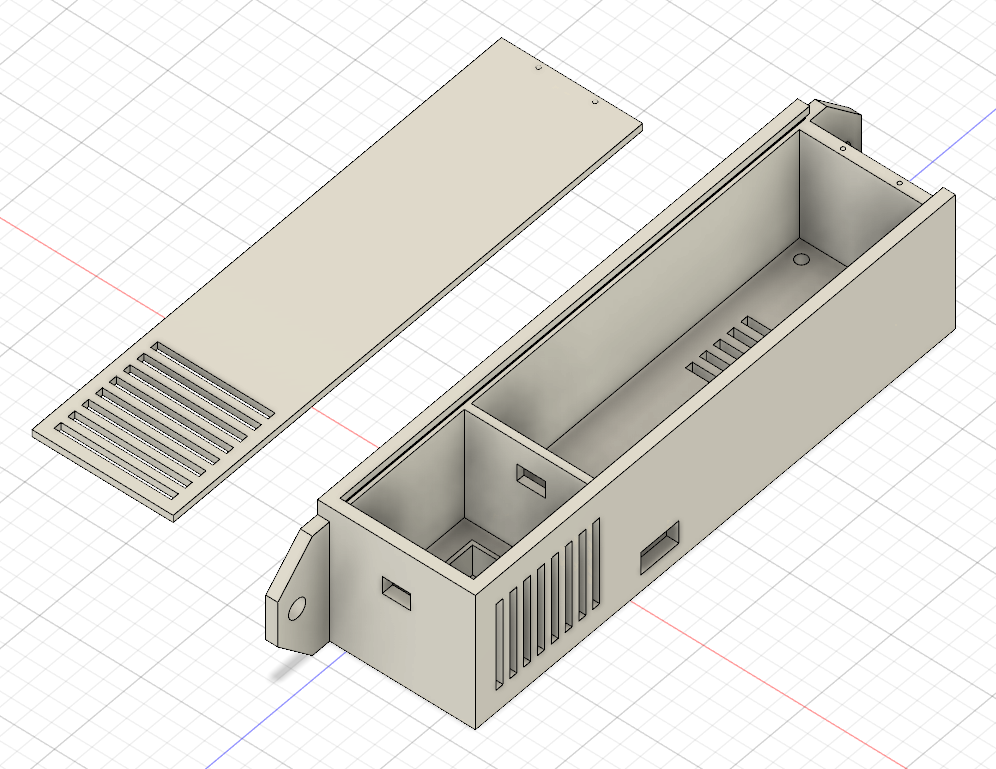
\includegraphics[width = (\textwidth)/2]{images/3d_case_model.png}
\caption{3D Modell unseres Gehäuses}
\label{fig:3d_case_model}
\end{figure}\\
Das Gehäuse bietet Löcher im Boden für eine Befestigung der Platine des Boards mittels Schrauben sowie eine separate Kammer innerhalb des Gehäuses mit Luftschlitzen für den Umgebungssensor. Der Deckel ist eine Schiebekonstruktion, da sich diese nach mehreren Iterationen bewährt hat und die eventuelle Abnutzung nicht dazu führen sollte, dass der Deckel nicht mehr auf dem Gehäuse hält. An den beiden Seiten befinden sich jeweils eine Bohrlasche zur Befestigung des Gehäuses an einer Wand. Es gibt ein Loch für die Führung von Kabeln nach außen, sowie eine Aussparung um den USB-Port des Boards.

\section{Ergebnisse}

\subsection{Funktionsumfang}
Wir haben funktionierende Prototypen, die mit bis zu 2 Fenstersensoren und einem Umweltsensor Daten an die Smart Home Zentrale senden. Die Knoten warten im Deep-Sleep auf einen Timer-Interrupt oder einen Interrupt von den Fenstersensoren. Die Smart Home Zentrale unterstützt beliebig viele Knoten mit Sensoren und stellt keine Beschränkung dar. Die Lost Node Detection sendet Benachrichtungen bei einem Ausfall und das Sicherheitssystem bei einem Ereignis im Alarmzustand. Ebenfalls funktioniert das automatische Aktivieren des Alarmzustandes beim Verlassen des Hauses. Das Stören des Funkkanals wurde nicht im realen Betrieb getestet. Bei entsprechenden Testdaten reagiert das System aber wie gewünscht.\\\\
Die Konfiguration des Systems konnte leider nicht so einfach gestaltet werden, wie wir uns das gewünscht hätten, aber durch die Shell und Fabric-Skripte ist der größte Teil abgefangen worden.\\

\subsection{Langzeittest}
Bisher wurde unser System nur auf die Korrektheit seiner Funktionalität getestet. Einem umfassenden Langzeittest wurde das System bisher aus zeitlichen Gründen noch nicht unterzogen. Lediglich ein durchgängiger Zeitraum von einer Woche wurde getestet. Bei diesem Test ist aufgefallen, dass das verwendete Board weitaus mehr Energie im Schlafmodus verbraucht, als geplant war und der Akku deshalb bereits nach einer Woche nicht mehr genug Energie zum Betrieb des Gerätes gespeichert hatte. Anstatt von 55 $\mu A$ verbraucht es etwa 15 mA im Deep Sleep\footnote{Hier genannte Verbrauchswerte wurden nicht von uns selbst gemessen, sondern einem Video von Andreas Spiess\cite{andreasSpiess} entnommen. Allerdings deckt sich unsere Berechnung der Akkulaufzeit von einer Woche mit dem Verbrauch von 15 mA. Unser Board ist in der ersten Zeile der Tabelle in den ersten Sekunden des Videos zu finden.}. Das wurde von uns keineswegs erwartet, vor allem da auf dem Board eine Halterung für einen Akku verbaut ist und von uns angenommen worden ist, dass es somit auf Akkubetrieb ausgelegt sein sollte. Unsere Vermutung ist es, dass der verbaute Spannungsregler für diesen Stromverbrauch verantwortlich ist.

\subsection{Gesamtkosten für das System}
Für das Gesamtsystem fallen geschätzt folgende Kosten\footnote{Die Kosten können abhängig von der Wahl des Bestellortes und evtl. Vergünstigungen durch den Erwerb größerer Mengen abweichen.} an:\\\\
\begin{tabularx}{\columnwidth}{p{5cm}|c|X}
\textbf{Systemkomponente} & \textbf{Stückzahl} & \textbf{Preis} \vspace{1mm}\\
\hline\hline
\textbf{Raspberry Pi 3} & & 60,00\euro{}\\
(inkl. WLAN, Bluetooth, Gehäuse, SD-Karte, Netzteil) & & \vspace{1mm}\\
\hline
\textbf{Wemos ESP32 Board} & 4 & 60,00\euro{}\\
(inkl. Li-Ion Batterie) & & \\
\hline
\textbf{Sensoren} & & 30,00\euro{}\\
Magnetsensoren & 8 &\\
BME280 & 4 & \\
oder BME680 & 4 & \\
\hline\hline
\textbf{Gesamt}: & & \textbf{150,00\euro{}}
\end{tabularx}
\\\\
Im Vergleich dazu kommen bei existierenden Smart Home Angeboten (hier: von der Firma \textit{innogy}) in etwa folgende Kosten zustande, die mehr als das doppelte der Gesamtkosten unseres Systems ausmachen:\footnote{https://www.innogy.com/web/cms/de/3749570/home/vorteile/sicher-wohnen/}\\\\
\begin{tabularx}{\columnwidth}{p{5cm}|c|X}
\textbf{Systemkomponente} & \textbf{Stückzahl} & \textbf{Preis}\vspace{1mm}\\
\hline\hline
\textbf{SmartHome Zentrale} & 1 & 99,95\euro{}\\
\hline
\textbf{Tür- und Fenstersensoren} & 8 & 239,60\euro{}\\
& (1) & (29,95\euro{})\\
\hline\hline
\textbf{Gesamt}: &  & \textbf{339,55\euro{}}
\end{tabularx}


\subsection{Fazit}
Insgesamt sind wir zufrieden mit dem Funktionsumfang und den Einstellungsmöglichkeiten unseres Projektes. Wir haben viel Zeit in Recherche gesetzt und waren teilweise sehr unzufrieden mit den am Markt angebotenen Lösungen. Wir sind aber überzeugt, dass unser Projekt die Anforderungen gut umgesetzt hat. Wir haben die komplette Kommunikation verschlüsselt und mit Zertifikaten abgesichert.\\
Die eingesetzten Kryptografieverfahren sind auf dem aktuellen Stand und bieten ausreichend Schutz. Wir haben das System vor gängigen Angriffen abgesichert und können bei Bedarf Benachrichtigungen senden. Die eingesetzte Software ist Open Source und unser Quellcode ist unter entsprechender Lizenz veröffentlicht.\\
Die Auswahl der Komponenten entspricht im Endeffekt unseren Wünschen, wobei wir noch nicht vollständig zufrieden mit den Boards sind. Unter anderem sind wir noch auf der Suche nach einer stromsparenderen Alternative zu unserem aktuellen ESP32 Board. Bei den Anschaffungs- und Erweiterungskosten sind wir unterhalb den kommerziellen Lösungen. Dabei sind unsere Knoten vielseitiger einsetzbar. Lediglich im Design und Kompaktheit können wir nicht mithalten, aber mit verbesserten und langzeiterprobten 3D-Druckvorlagen könnten wir aufschließen.

\section{Ausblick}
Es wird ein Langzeittest des Systems folgen, anhand dessen das System optimiert werden kann und eventuelle Probleme behoben werden können.\\
Aktuell wird an einer Portierung\footnote{Im Repository\cite{smarthome2} unter dem Branch \textit{riot\_port}} der Anwendung für den ESP32 auf RIOT gearbeitet, was allerdings nicht mehr Teil dieses Softwareprojektes ist. Es bleibt abzuwarten, in welchem Umfang die Anwendung portiert werden kann, da die Portierung des ESP32 auf RIOT selbst noch nicht abgeschlossen ist\footnote{\url{https://github.com/gschorcht/RIOT-Xtensa-ESP/wiki/ESP32-port}. Stand vom 26.07.2018}. Eine der wichtigsten fehlenden Features des RIOT-Ports ist derzeit die Implementierung des Deep Sleep. Ohne dessen Implementierung ist der Betrieb über einen Akku aussichtslos und nur über feste Stromversorgung möglich.\\\\
Es ist naheliegend, dass wir in Zukunft auch weitere Sicherheitsfunktionen hinzufügen, um auf kommerzielle Produkte aufzuschließen. Dazu käme die Integration von Kameras und Bewegungsmeldern, um einen detaillierteren Eindruck über das Geschehen im Haus zu erlangen. Zur Sicherheit gehört nicht nur der Schutz vor Einbrüchen, sondern auch vor Gefahren für das Haus und dessen Bewohner. Wir haben mit den Umweltsensoren bereits angefangen, wobei der BME680 sogar in der Lage ist, flüchtige Gase zu erkennen, aber weitere Sensoren, wie etwa Brandmelder oder Wassersensoren, die eine auslaufende Waschmaschine, Heizung oder Geschirrspüler erkennen, fehlen derzeit noch.

\nocite{*}
\bibliographystyle{unsrt}
\bibliography{bibliographie}
\end{document}
